%%% Bareme

\setlength{\marginparpush}{2pt}
\newcounter{totalpointsint}
\newcounter{tempsint}
\setcounter{totalpointsint}{0}
\newcounter{minutesparpoint}
\newcounter{degresint}
\newcounter{anglefancyclock}
\newcounter{dureeexamheures}
\newcommand{\BaremeSurTroisH}{
\setcounter{minutesparpoint}{9}
\setcounter{dureeexamheures}{3}
}
\newcommand{\BaremeSurDeuxH}{
\setcounter{minutesparpoint}{6}
\setcounter{dureeexamheures}{2}
}
\newcommand{\DebutBareme}{
\setcounter{anglefancyclock}{90}
}
\setcounter{minutesparpoint}{1}
%\BaremeSurTroisH
\DebutBareme
\newcommand{\fancyclockmin}[1]{
\setcounter{tempsint}{\theminutesparpoint*\real{#1}}
\setcounter{degresint}{\thetempsint*6}
\setcounter{anglefancyclock}{\theanglefancyclock-\thedegresint}
\noindent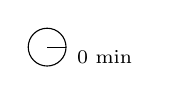
\begin{tikzpicture}[scale=.8]
    \draw (0,0) circle (3mm);
\ifnum\theanglefancyclock<0          % modulo de l'angle
\addtocounter{anglefancyclock}{360}  %
\fi                                  %
%\draw (0mm,0mm) node [black!30] {\bf\Large\thedureeexamheures};
%\draw (0mm,0mm) node [black!25] {\Large\thedureeexamheures};
\filldraw[rotate=\theanglefancyclock] (0,0) -- (0:3mm) arc (0:\thedegresint:3mm) -- cycle;
%\draw (3.2mm, 1.5mm) node[anchor=west] {\scriptsize #1~pt};
\draw (3.2mm, -1.5mm) node[anchor=west] {\scriptsize \thetempsint~min};
  \end{tikzpicture}
% \tiny
% \begin{tabular}{@{}r@{} @{}l@{}}
%  #1&~pt\\
%  \thetempsint&~min
% \end{tabular}
}

\newcommand{\bareme}[1]{%
\addtocounter{totalpointsint}{10*\real{#1}}\marginpar{%
\footnotesize\fancyclockmin{#1}
%\hfill\thetotalpointsint
}}
\newcommand{\Bareme}[1]{\marginpar{\fbox{\small tot: #1 pt}\hfill}}
